\chapter{An Apparatus To Compare Energy Usage}
\label{chapter:testrig}

As discovered in \autoref{section:literature}, it is still uncommon to routinely compare the energy usage due to different software, both when selecting existing applications or components and when creating or maintaining new software. This chapter describes the design and construction of a prototype low-cost apparatus to allow software energy usage comparisons to be included in the regular software testing process. The prototype apparatus was evaluated by comparing the energy usage and performance of a range of web server software. In \autoref{chapter:comp energy} the apparatus is also used to compare the energy usage of the components from \autoref{chapter:performance}.

\section{Introduction}
\label{section:rig introduction}

The previous chapters have led to several important conclusions.

\begin{itemize}
\item The energy consumption of the internet is very large, and for sustainability this needs to be reduced.
\item Software systems are a key factor in the energy consumption of the internet.
\item Software systems vary widely in performance, even when performing the same task.
\item Information is generally not provided about the energy-efficiency of software.
\end{itemize}

These conclusions in turn lead to the hypothesis that the energy usage of a components and applications may vary in energy use. If true this implies that the energy use of web software system may potentially be reduced by replacing components with functionally equivalent components which use less energy. In order to verify this initial hypothesis, a prototype apparatus was developed to measure and compare the energy usage of different applications, servers, and software components, and therefore to determine whether the overall energy usage of server-side web software applications could be reduced.

\section{Existing Approaches}

Attempting to determine the efficiency and energy usage of computer systems is not a new idea. What is new is the increasing realisation of the large environmental and climate impact of the world's computer systems and the corresponding desire to reduce that impact as much as possible, as soon as possible. This goal requires a holistic approach considering all aspects of the global computing ecosystem. This section provides an overview of existing approaches and research.

The largest and most diverse category of research into energy usage is that of electronics and computing hardware. This is with good reason. It is the physical electrical and electronic parts of the systems which consume energy in order to function and produce heat which requires cooling. Electronic components and subsystems are commonly provided with \emph{data sheets} which include vital information such as voltage and current requirements, power dissipation, and operating temperature ranges. Manufacturers compete on optimising these numbers, and each new generation of technology often results in a general improvement. Reducing the overall energy requirements of the physical components which make up computing systems is an important way to reduce global energy usage and its associated greenhouse gas emissions.

Unfortunately, measuring the energy usage of electronic infrastructure is the point at which much existing research stops. Although built from electrical and electronic components, computer systems are not simple electrical systems which can be understood as a mathematical function of their components. The power consumption of a computer processor, and by implication the whole computer system, can vary by hundreds of watts depending on the software running at the time \citep{derBauer2023}. Software also influences the power consumption of memory, storage, networking, and other computing facilities \citep{Basmadjian2012}.

However, software \emph{changes}. The reason that software-defined systems are so different from pure electronic solutions is the ability to change and update the behaviour of a system without changing the hardware. When attempting to determine the energy usage of a programmable system, it needs to be re-evaluated every time the software changes. Depending on the software development process in use, that can be many times per day \citep{Shahin2017}. As was shown in \autoref{section:fs1}, small changes can have a big impact. In an ideal scenario, whatever method is used to determine any increases or decreases in energy usage should integrate seamlessly into the software development process alongside tests for correct function and performance.

Many mobile and portable devices rely on batteries for power. The trade-off between weight, size, and battery capacity means that these devices  have limited energy availability, and need to conserve energy wherever possible. Testing, and reducing, energy consumption is a key part of the design process for both hardware and software in battery-operated systems. Software which causes too great a battery drain is not fit for purpose. The simplest way to determine the energy usage of such devices is to measure how long they can continue operating before the battery is drained \citep{Brown2006}. This form of measurement, while arguably representative of real-world usage, is relatively coarse. Battery behaviour is complex \citep{Panigrahi2001} and it can be difficult to find what is causing the problem when battery life is not as expected. Such battery life testing is, by its nature, not a quick process. Testing multiple usage scenarios can be prohibitively lengthy, and is therefore not really suitable for frequent automated testing.

A common way to measure the operational energy usage of any electronic system is connect a meter and observe the results \citep{derBauer2023}. This approach has the advantage of simplicity and familiarity to anyone with an electrical or electronics background. Such meters are generally available at relatively low cost and easy to connect in the power supply to the device being tested. There are several drawbacks to this approach, however, which make it less suitable for comparing the energy consumption of different software or different versions of the same software. A major issue is that it is a manual measurement, and requires a skilled observer. This does not integrate well with automated tests run many times a day, and is a challenge for geographically distributed teams. Manual measurement can also miss transient events which might lead to a miscalculation of the real usage. On the whole, while this approach is better than nothing, it is neither accurate, repeatable, nor easily automated. Electronics manufacturers are aware of the problems of manual measurements on complex systems. Test and measurement equipment models are available which offer data logging, communication with other devices using a variety of protocols, and other complex features. Such test equipment is considerably more expensive than manually-operated equipment, though. 

Computer component manufacturers are also aware of this problem, and some include power-measurement circuitry in processors or supporting chipsets. For example, modern processors from Intel include \emph{Running Average Power Limit} (RAPL) circuitry which may be queried by software to determine the power consumption of specific components of the computer system \citep{Travers2015} \citep{Hahnel2012}. In some scenarios, such as software which is very processor-intensive, this can be an effective solution, particularly when the measurement facilities are already included in the computer hardware being used for development, testing, and deployment of the software. This approach does have its disadvantages, however. The power measurement is not holistic, and may not include energy used by other components such as storage drives, cooling fans and network interfaces which are not part of the central processor or its supporting chipset. There is also the problem that the measurement and control software is being run on the same device, and its energy usage will be merged with the energy usage of the software which is being tested. In cases where the software under test uses a large proportion of the available computing facilities, the overhead of the test and measurement software will be small in proportion, but in scenarios with a wider range of software this can act to confuse the measurements.

If the software is deployed to a cloud hosting service, or co-located in a datacenter, the hosting partner may be able to provide some form of power usage information. Where available, this is typically aggregated across all the services in a project or all services hosted for a particular client. This kind of power consumption measurement has the advantage of being holistic, in that it includes power supplies and their associated losses as well as processors, memory, storage drives, cooling fans, network interfaces, and all the other equipment required to keep an internet service running. The disadvantage is its coarse-grained nature. Although data from such power consumption measurements can be used to track trends and indicate major increases or decreases in overall energy use, it is rarely precise enough to identify the contribution due to individual software.

In many commercial projects, there is no attempt to measure energy usage directly. Instead, monetary cost is used as a proxy. If the energy cost for running a project or service increases, then it is treated as if the project is using more energy, and vice versa. This approach has the advantage of fitting naturally with the information used to manage the financial aspects of a business. Unfortunately, it has all the disadvantages of hosting service measurements with the added complexity of changing energy prices. If this approach is then used to determine greenhouse gas emissions, it is also subject to strategies such as `carbon offsetting' which can make it appear that a product, project, or service is `greener' that it is.

The above approaches are not exclusive, and many combinations are possible. For example, both \citet{Kaup2014} and \citet{Stoico2023} used an aggregated performance modelling approach in conjunction with a commercial external power measurement device to estimate energy usage in a variety of scenarios.

\section{Research Gap}

The existing approaches mentioned above have a mixture of advantages and disadvantages, but none quite fit the needs of a software development team which frequently and automatically tests individual services and complete systems during development to ensure that the end result meets requirements and is free of faults before deployment. This technique is known as `Continuous Integration' (CI) \citep{Meyer2014} and is very popular in conjunction with agile development practices \citep{Shahin2017}. An ideal solution for this situation would include the following features:

\begin{itemize}
\item Support testing of existing software without manual modification or substantive changes
\item Measure the energy consumption of the whole system, not just certain components
\item Measure energy consumption during representative usage
\item Be precise enough and fast enough to catch transient events
\item Be programmable so it can be used in a CI build process
\item Be able to operate repeatedly without human intervention
\end{itemize}

The following sections describe the design, construction, and testing of a prototype apparatus to address these requirements.

\section{Methods and Prototype Apparatus}

The apparatus described is a research prototype, developed on a small scale and to a low budget. Future implementations could revisit the architectural decisions, particularly the choice of power measurement and server hardware. Potential improvements and future possibilities are discussed in \autoref{Improvements}.

\subsection{Solution Architecture}

The key elements of the architecture are a computer platform on which to install the software to be tested (DUT), a way of measuring the power used by that platform, and one (or more) computers to act as clients and make requests to exercise the software (LOAD). This system also includes a separate computer to manage the operation of the apparatus and interface with the power measurement device (CTRL), and a separate server containing a database for data logging (LOG). All these systems are connected by a local network which can be separate from the internet during normal operation.

\begin{figure}[htbp]
  \centering
  % \def\svgwidth{\columnwidth}
  \includesvg[width=\columnwidth]{Figures/rig/rig.svg}
  \caption{Prototype Apparatus System Diagram}
\end{figure}

\subsection{Power Measurement Technology}
\label{Power measurement}

During the construction of the prototype a range of power measurement technologies were considered (see \autoref{literature:methods}), eventually settling on the INA260 chip from Texas Instruments \citep{TexasInstruments2016} which can work with DC voltages up to 36V and currents up to 15A. This was purchased in the form of a pre-built evaluation board from Adafruit \citep{AdafruitINA260}. The INA260 is controlled using 12C with a default address of 0x48. In this apparatus SDA and SCL lines are connected to an i2C interface on the CTRL device.

The INA260 is capable of both `high side' (in series with the positive voltage to the DUT) and `low side' (in series with the ground connection) measurements. In its  default configuration, the most accurate readings are gained when used in a high side circuit \citep{TexasInstruments2016}, so the Adafruit board was connected in the high side of the power supplied to the DUT device. Adafruit provide a Python library for the control and measurement of this board which was used when building the control software for the apparatus.

\subsection{Computer Hardware}

The choice of power measurement hardware influenced the choice of computer platform. Any computer used for the DUT device would need to be DC powered  and consume no more than 36V and 15A. A popular choice for research is the \emph{Raspberry Pi} single-board computer \citep{RaspberryPi}, which fits the required power supply range.

The Raspberry Pi computer is based on an ARM CPU \citep{ARM} manufactured under license by Broadcom and has various models with different CPU variants and memory sizes. The specific board chosen for the DUT device in this prototype was a Raspberry Pi 4 Model B with 8 GB of memory. Although the computer is physically small, it is capable of running much of the same software as larger and more power-hungry server systems \citep{Varghese2015}. To ensure that the DUT device would not just be idling during tests, a similar computer is used for the LOAD device. Although the architecture supports multiple LOAD devices, only one was implemented in this prototype. Software to simulate client interactions with a service is typically less resource-intensive than the service itself, so this was not considered to be a major issue.

For simplicity the CTRL device also used a Raspberry Pi. This role did not need such a high specification, so a cheaper Raspberry Pi 3 Model B with 4GB RAM was chosen. 

\begin{figure}[htbp]
  \centering
  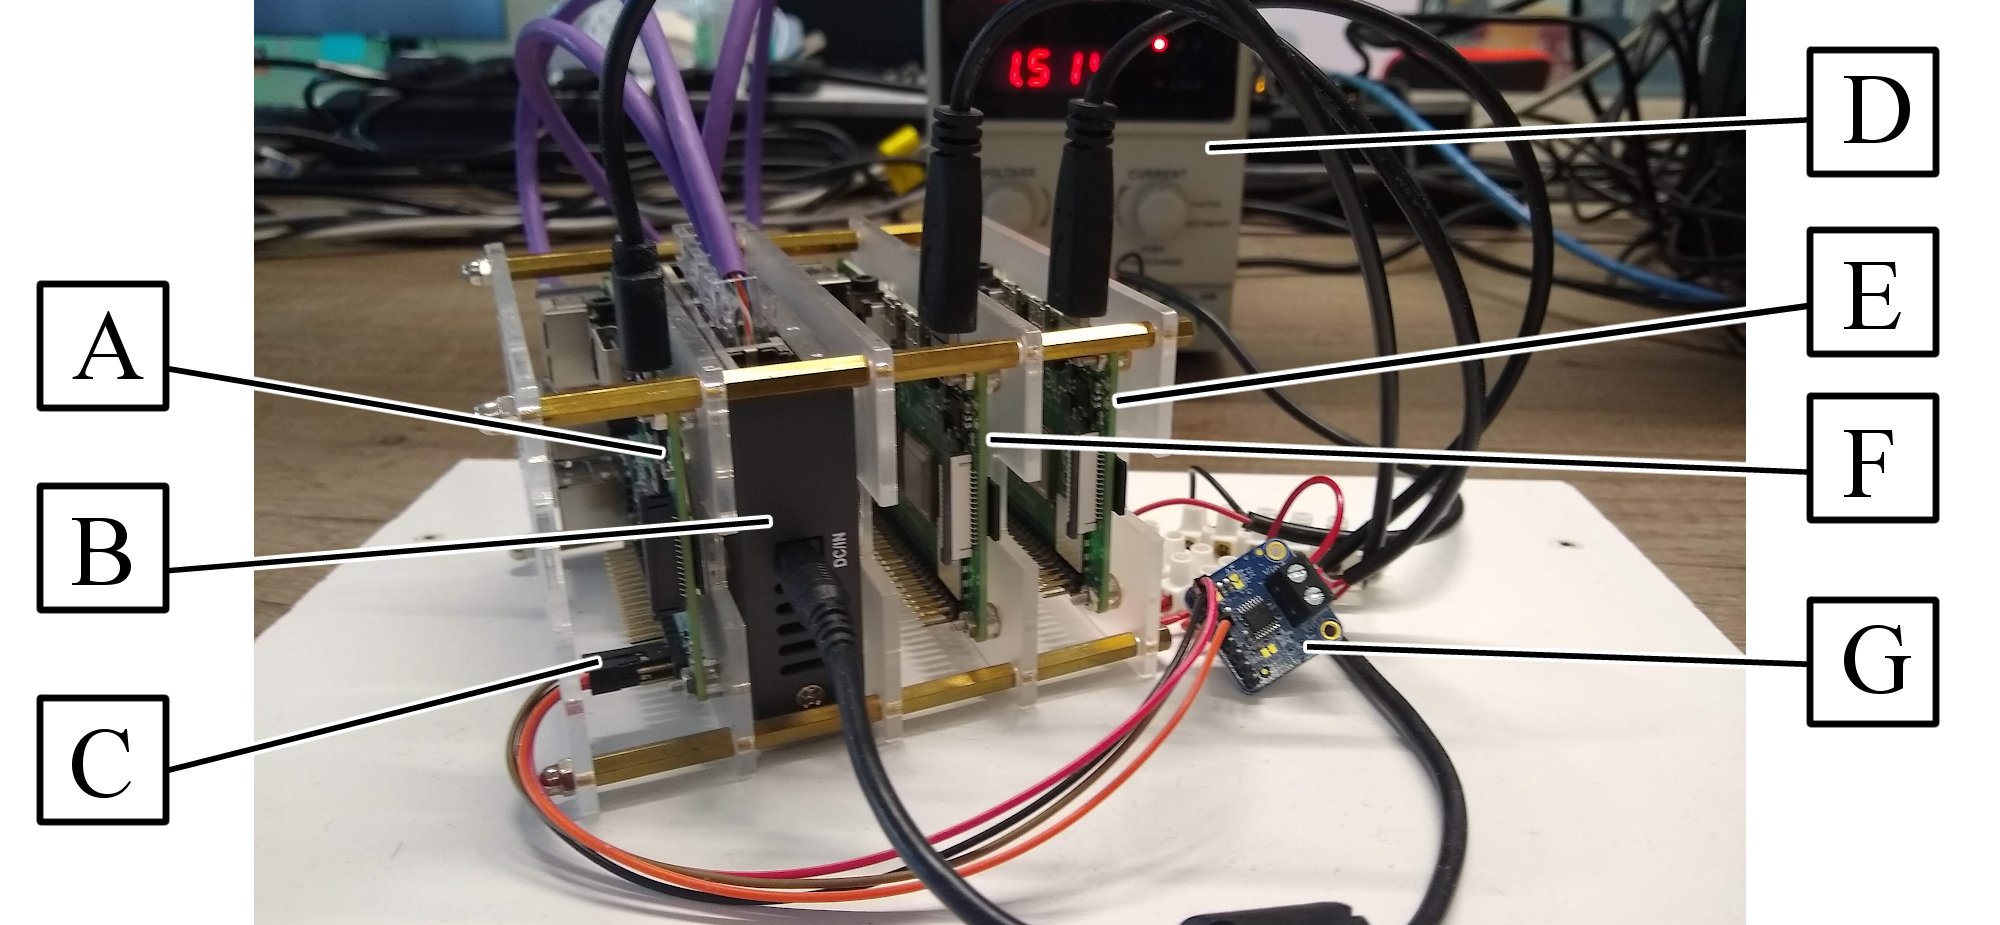
\includegraphics[width=\columnwidth]{Figures/rig/testrig-annotated-1.png}
  \label{hardware}
  \begin{tabular}{|ll|}
  \hline
                                   & \textbf{D} \quad 5V Power Supply \\
  \textbf{A} \quad CTRL Device     & \textbf{E} \quad DUT Device \\
  \textbf{B} \quad Network Switch  & \textbf{F} \quad LOAD Device \\
  \textbf{C} \quad I2C Connector   & \textbf{G} \quad INA260 Board \\
  \hline
  \end{tabular}
  \caption{Prototype Hardware}
\end{figure}

In all cases the computers used a variant of the Debian Linux operating system.

\subsection{Data Logging}

The machine used for data logging needed larger and faster data storage than available on a Raspberry Pi, so a generic Intel-based desktop PC was chosen. The logging system consists of two main software components: A PostgreSQL database and a service to receive data from the CTRL device and store it in the database. The data logging service provides a REST \citep{Fielding2000} interface for the CTRL device to submit experiment status and progress data as well as measurements from the INA260. 

For near-real-time data visualisation during experiments a Grafana dashboard \citep{Grafana} was configured to read, aggregate, and display power usage data every second from the database. Data gathered during experiments remains in the database for subsequent analysis.

\subsection{Power and Networking}

As discussed in \autoref{Power measurement}, the selected power measurement technology only works with DC voltages. While this is perfect for the Raspberry Pi boards, which all work with 5V DC power, it is not suitable for traditional desktop computers which require an AC supply from which they generate DC voltages appropriate to the different parts of the system. For this reason the prototype apparatus uses two separate power sources: a stable 5V DC supply for the Raspberry Pi devices and an AC supply for the data logging server.

All the computing devices needed to be networked together, so in this prototype, a low-cost, low-power, 5-port gigabit switch is mounted alongside the Raspberry Pi devices. The ports link the three Raspberry Pi devices and the logging server as well as providing an `uplink' to a network with PCs for software development, debugging and results analysis. The selected network switch also requires 5V DC power, and is powered by the same supply as the Raspberry Pis.

\subsection{System configuration}

Each participating computer needs to know the IP addresses and ports of any other services it makes use of. Early versions of the prototype were manually configured using a simple key-value text file. This rapidly became cumbersome when using the system with other networks with different IP allocation rules. It also became a problem whenever one of the participating computers needed to be replaced or re-installed.

To overcome this issue a service registry was added which provided a single point of access for whatever services were added to the system. This registry functions in a similar way to Eureka \citep{Netflix2012}. On start-up, every service registers itself with the registry and receives a \emph{lease} with a limited duration. The service must renew this lease before expiry or be removed from the registry. This leasing process keeps the list of services \enquote{fresh} \citep{Arnold1999} and reduces the risk of attempting to connect to an obsolete or unavailable service. When one service needs to communicate with another, it requests details of the endpoint from the service registry.

To minimise the number of separate machines in the system, the service registry is installed on the LOG system. This machine is allocated a static IP address, so that a fresh installation of any of the other participants can find the server, register, and obtain IP addresses and ports of the other participating services, even in a DHCP environment where IP addresses may not be consistent.

\subsection{Software installation and version control}

As well as simplifying the hardware, the choice to use similar devices for the DUT, LOAD, and CTRL roles made it possible to use a single `disc' image for all three participants. The Raspberry Pi has no hard drive or SSD storage in the usual sense, but instead uses an SD card. While this approach has some issues with performance and reliability (see \autoref{limitations}), it has the advantages that the cards are removable and relatively easy to copy. During development a single `golden' card image was maintained containing up-to-date versions of all the services. Whenever a card became corrupted, failed, or otherwise needed replacing, it was a simple matter of copying the golden card image.

While basing all the Raspberry Pi systems on the same image made version management and failure recovery much simpler than a completely manual configuration, there was still one more step required. When the system starts it needs to know which role it should perform. In the current prototype, this information is contained in a plain text file at a known location on the card image, and must be manually edited before booting the Raspberry Pi device. Other approaches are potentially available to avoid the need for this, and are discussed in \autoref{Improvements}.

\subsection{Preparation}
\label{Preparation}

In operation, the apparatus involves dynamic participation by services running on all four of the main hardware components (CTRL, DUT, LOAD, and LOG). Before measurement can start, however, the system needs to be configured for the specific measurements. This proceeds in four steps, which can be done either manually (via SSH terminal sessions to the appropriate devices) or under control of a CI build system which has remote access to the devices.

\begin{enumerate}

\item  Install the software to be tested. When comparing external applications this process will usually involve installing the applications according to their specific instructions, but may involve the same `Infrastructure-as-code' tools such as \emph{Ansible}\footnote{\url{https://www.ansible.com/}}, \emph{Chef}\footnote{\url{https://www.chef.io/}}, \emph{Puppet}\footnote{\url{https://www.puppet.com/}}, or \emph{Terraform}\footnote{\url{https://www.terraform.io/}} which would be used to deploy the application for real \citep{Rahman2019}. When comparing versions of an internal application, this process may also include fetching the software from a code repository such as \emph{GitHub}.

\item Create scripts for the apparatus to use to start and stop the software. These scripts have standard names and locations known to the measurement software and enable the system to start and stop arbitrarily complex installations without the need to modify the measurement software itself. As will be seen in \autoref{Measurement}, these scripts not only start and stop the software, but also notify the measurement controller when start-up and shut-down is complete, to support the measurement of software with lengthy or complex start-up and shut-down behaviour.

\item Configure the client service on the LOAD device. When evaluating this prototype, client requests were simulated using the \emph{Siege}\footnote{\url{https://github.com/JoeDog/siege}} load testing tool so the configuration consists of creating a script to call \emph{Siege} and to notify the measurement controller when it has finished. \emph{Siege} was selected after an examination of several alternatives. Many popular load testing tools such as \emph{JMeter}\footnote{\url{https://jmeter.apache.org/}} and \emph{Locust}\footnote{\url{https://locust.io/}} are designed for programmable scripting and performance testing of specific HTTP requests. For realistic comparison of energy use it is important to emulate a web browser which automatically fetches any associated page resources such as images, CSS, and JavaScript. \emph{Siege} does this and is easy to control with command-line parameters. The process of selecting and evaluating potential load testing tools was not exhaustive, for reasons explained in \autoref{fs1:intro}.

\item Provide the measurement system with identifying information about the upcoming measurement so that the resulting data can be retrieved from the database when the measurement is completed. Typically this information is in the form of a textual name and a version or sequence number. The identifying information can be provided either manually using a web form, or by the CI process using an HTTP API.

\end{enumerate}

\subsection{Measurement Operation}
\label{Measurement}

Once preparation and software installation is complete, measurement is started either by a user clicking on a button on the CTRL web interface (\autoref{Web UI CTRL}), or by an API request from a CI process. The apparatus then runs a sequence of operations managed by the CTRL device, as shown in \autoref{Sequence Diagram}.

\begin{figure}[htbp]
  \centering
  \includesvg{Figures/rig/sequence.svg}
  \caption{Measurement operation sequence diagram}
  \label{Sequence Diagram}
\end{figure}

The sequence begins by notifying the LOG that a measurement is starting, which enables it to group subsequent measurements together as a single experiment for later analysis. Following this, \emph{Warmup} instructions are sent to DUT and LOAD. These start the services using the scripts described in \autoref{Preparation}, which in turn notify CTRL when they are complete. When both DUT and LOAD are ready, the first of two phases of measurement begins.

Computers are complex systems and the amount of power they use, even when not explicitly running application software, can vary due to a range of factors, including ambient temperature \citep{Jin2022}, operating system software versions and updates \citep{Williams2015}, network activity \citep{Canek2022}, and other time or environmental factors. To eliminate as much of this variability as possible, the apparatus runs an initial phase of measurement with no LOAD activity which is then used as a \emph{baseline} for the measurements under load which follow. LOG is also notified of the start and end of this baseline measurement phase, so that these measurements are not confused with the active phase.

When the baseline measurements are completed, the second, active, phase begins. LOG is notified to expect active readings, the LOAD process starts, and readings are collected until LOAD reports that it is complete, at which point LOG is notified that the experiment is ended. All messages to LOG are timestamped so that the length of time taken to service the load can also be included in the analysis. Finally \emph{Cooldown} instructions are sent to DUT and LOAD to revert changes made during \emph{Warmup}, if required.

Execution time for the whole measurement cycle varies depending on the choice of load and the requirements and capabilities of the software being investigated. During validation of this prototype, the duration of each measurement cycle was typically of the order of a few minutes.

\subsection{External Interfaces}
\label{Web UI}

Each of the platforms which comprise the comparison apparatus provide multiple ways for external software to interact with them. To enable automated installation and configuration of services to be compared and client software to exercise them, the DUT and LOAD devices provide secure shell (ssh) access. Software installation and removal often requires superuser privileges, so this is also available to authenticated ssh users. This ssh access is also used by the CTRL device when it calls the \emph{Warmup}, \emph{Cooldown}, \emph{Start}, and \emph{Stop} scripts to manage comparison runs. Such access comes with significant risk, however. Accidental or malicious commands over this channel could damage the operating system or the software which operates the DUT and LOAD services or even install other malicious or exploitative software on the apparatus. The risk of this is mitigated somewhat by two factors. The first factor is the isolation of the apparatus from other networks except when required to install software, and the second is the easy and regular re-installation of each system from an externally-created and managed `golden' disk image. In most cases for this prototype it is both simpler and safer to start each group of tests from a fresh disc image rather than relying on a clean de-installation of a previous candidate.

The REGISTRY, CTRL, and LOG systems all provide safer interaction mechanisms in the form of REST interfaces for use by integration testing software and web interfaces for manual use by humans. In each case the web interface is mainly just a wrapper around the REST requests. All operations provided by the web interfaces can also be achieved by calls to the REST API.

\subsubsection{Registry Web Interface}
\label{Web UI Registry}

A screenshot of the web interface for the registry is shown in \autoref{UI registry}. At the top is a table of the currently registered devices in the system with their IP addresses, the remaining time before their leases need to be renewed, and a set of options for each one to deregister, remove and shutdown individual services. This table is automatically refreshed using JavaScript, but should that fail for some reason there is also a `link button' to force a refresh of the table.

\begin{figure}[ht!]
\centering
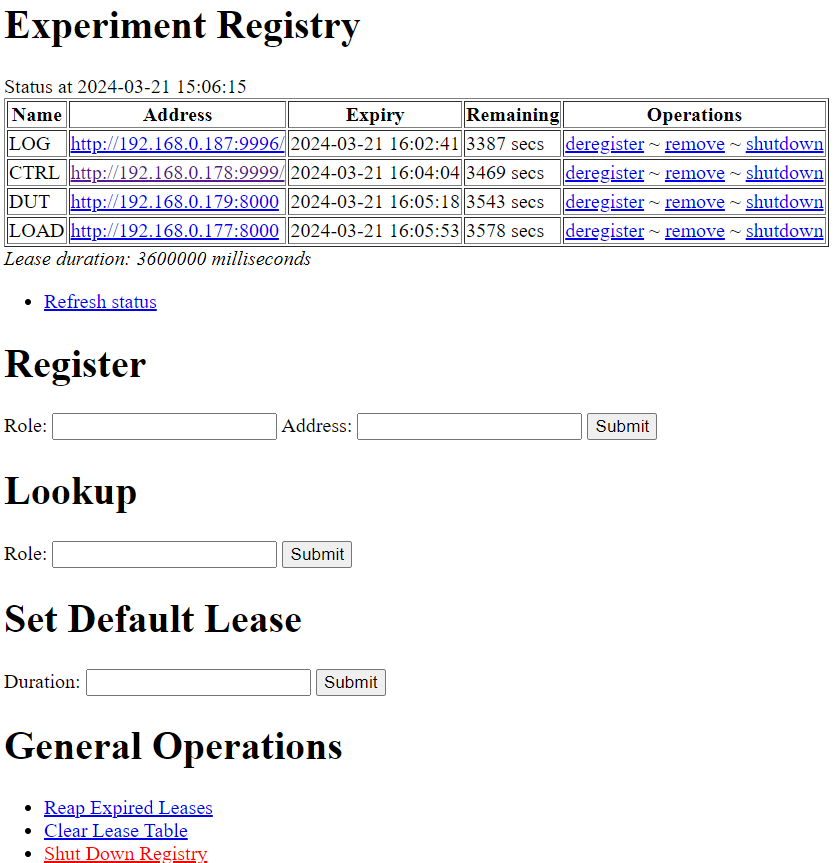
\includegraphics[width=\columnwidth]{Figures/screenshots/Registry.png}
\caption{Web Interface to the Registry}
\label{UI registry}
\end{figure}

The web registry interface also includes a form for manually registering a device. This is typically only used for testing, to check that the `lookup' process is working correctly, because it does not set anything running which will renew the lease when it expires. Also used for system testing is a form which calls the REST endpoint used for looking up the IP address of a device. The final form on this page allows setting the duration of future leases. By default, the system issues leases valid for 1 hour (3,600,000 milliseconds) but when stopping, starting, or replacing devices or services, it can be useful to set the lease expiry to a shorter value.

In addition to the forms, the registry interface also includes `link buttons' which remove expired leases (typically from devices which have been replaced and gained a new IP address), clear the whole lease table, and shutdown the registry service.

All the forms and buttons one ach of the web interfaces have attached JavaScript code which shows a temporary message to confirm success or failure of the operation.

\subsubsection{CTRL Web Interface}
\label{Web UI CTRL}

A screenshot of the web interface for the CTRL role is shown in \autoref{UI CTRL}. At the top is a status display for the currently running experiment. `running' is true when an energy measurement is in operation. `child' indicates the status of the process which interacts with the INA260 device over the I2C interface. This process is started at the beginning of each experiment and shutdown at the end. `dut\_ready' and `load\_ready' indicate whether the relevant service has confirmed completion of its \emph{Warmup} script. `scenario' and `session' reflect the information entered for the current experiment.

\begin{figure}[ht!]
\centering
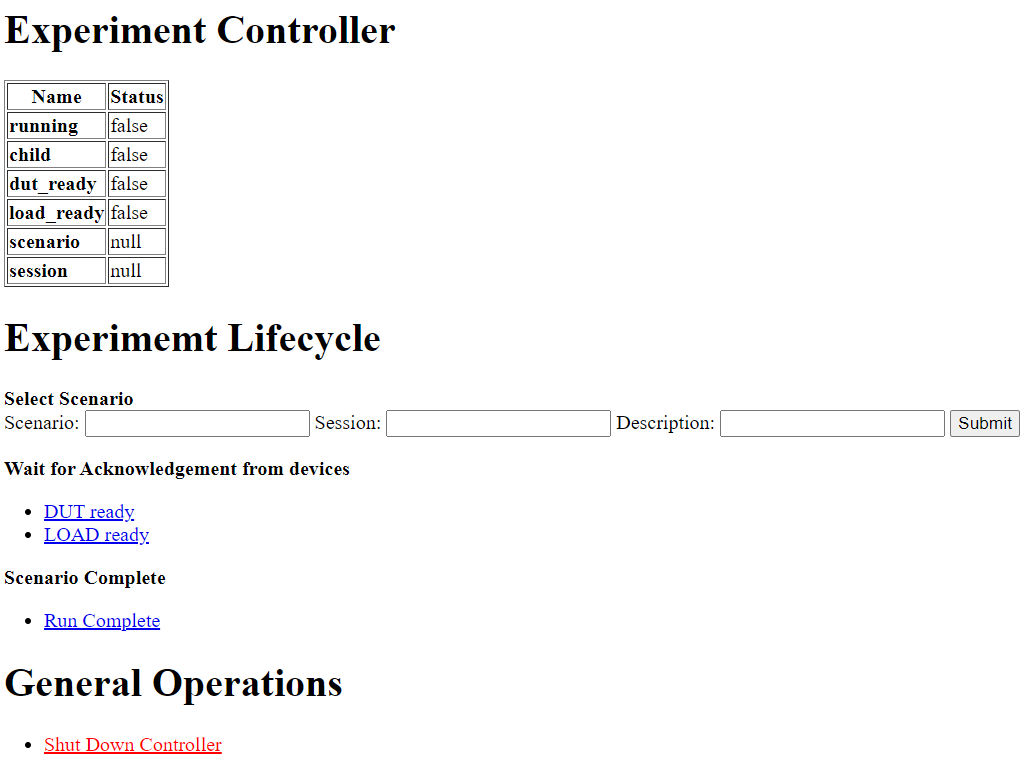
\includegraphics[width=\columnwidth]{Figures/screenshots/Controller.png}
\caption{Web Interface to the Experiment Controller}
\label{UI CTRL}
\end{figure}

An experiment is started by entering a scenario name and a session number for that scenario and clicking `Submit'. These values are separate to make identification easier when executing multiple runs of a single scenario for averaging. There is also an optional field for some descriptive text which will be stored in the database with the details of the experiment but has no automated use. As the experiment progresses, the values in the status display are updated.

For testing purposes the CTRL interface also provides `link buttons' to manually trigger the normally-automated responses from the DUT and LOAD devices, as well as a way to manually mark a run as complete. These options can be useful when testing that the software to be measured is installed correctly and that valid \emph{Warmup}, \emph{Cooldown}, \emph{Start}, and \emph{Stop} scripts have been created and placed in the correct places. The `Run Complete' button is particularly useful if an experiment fails to terminate and is continuing to send data to the LOG service and the database.

Just as with the other interfaces, the CTRL interface also provides a button to shut down the CTRL service.

\subsubsection{LOG Web Interface}
\label{Web UI LOG}

A screenshot of the web interface to the LOG role is shown in \autoref{UI LOG}. At the top is diagnostic information about the current active session, if any, and the current number of stored readings from the INA260 in the \verb!log! table.. The database consists of two active tables: \verb!log!, in which each row is a single timestamped voltage and current reading from the INA260; and \verb!session2!, in which each row describes a measurement session with its scenario name, session number and description, as well as the starting and ending timestamps for the `baseline' and `active' readings. The SQL creation script for the database is given in \autoref{appendix:database}.

\begin{figure}[ht!]
\centering
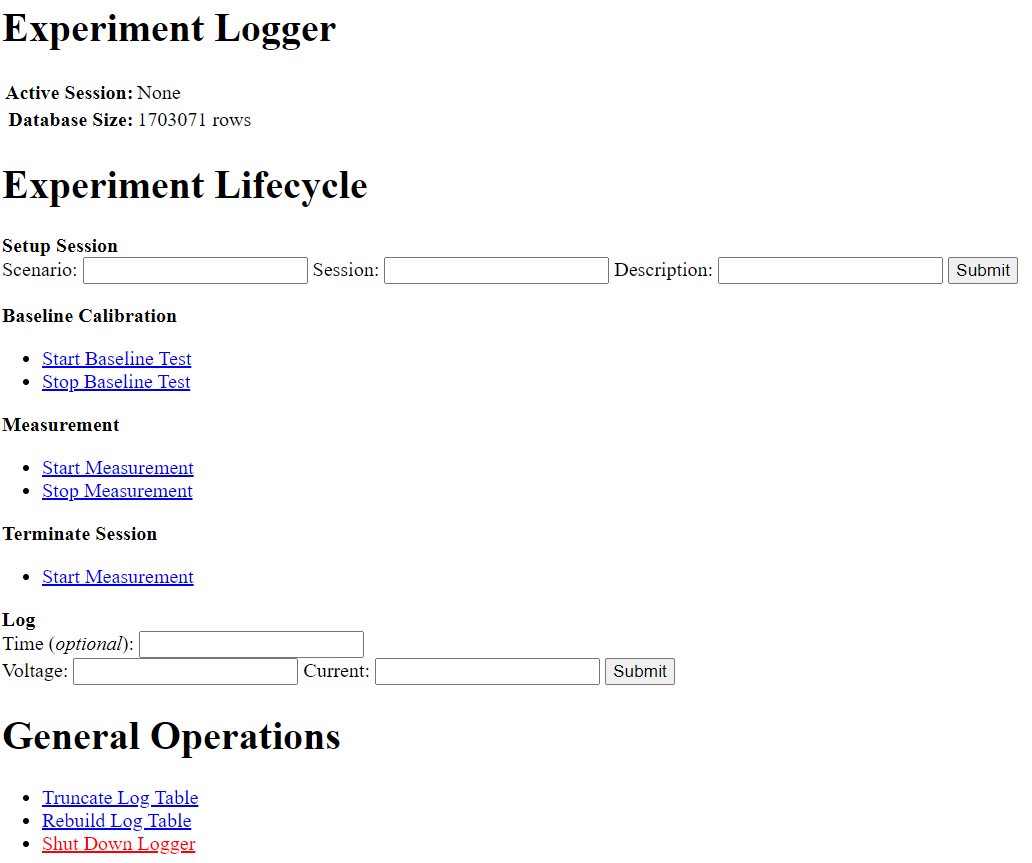
\includegraphics[width=\columnwidth]{Figures/screenshots/Logger.png}
\caption{Web Interface to the Experiment Logger}
\label{UI LOG}
\end{figure}

The LOG web interface provides a form to create a session in the \verb!scenario2! table and some `link buttons' to set the start and end timestamps for the `baseline' and `active' readings. There is also a button to manually terminate a session, but in this version of the prototype this button is mis-labelled. In addition to the buttons which add data into the \verb!scenario2! table, there is also a form to manually enter some dummy readings for test purposes. This form requires voltage and current values and an optional timestamp. If no timestamp is provided, the current time is used.

As with the other services, the LOG interface provides general administration functions to truncate or rebuild the \verb!log! table and to shutdown the LOG service.

\section{Results and Analysis}

\subsection{Validation of the Design}
\label{validation}

To validate the design of the apparatus, it was needed to show that the power measurement circuitry will generate different readings when different software is in operation. The same approach as \citet{Kaup2014} was taken, by creating a simple `infinite loop' which could be run from a terminal session connected to the DUT machine. With the CTRL and LOG software running, the measurements on the Grafana dashboard were observed when the loop was not running and when it was running. There was a clear difference, which can be seen in \autoref{Run 1}. The readings are not consistent in this graph, and exhibit some `glitches'. This is due to the manual nature of the tests. For example, the drop in energy usage at around 16:48 shows the point at which the loop code was changed so that it no longer `printed' a message to the (remote) console every cycle. This shows an overall reduction in energy use by both the CPU and the network hardware. Note also that the peak power usage is around 2.5W (or 2.4W without the `print') for this run. Even though the code was running an infinite loop, which should cause the processor to work as hard as it can, the peak power usage is less than some of the readings from real application tests in \autoref{comparisons}. A hypothesis is that this occurs because the loop used in this test is only exercising a single core of the CPU, as  observed by \citet{Basmadjian2012}. The applications investigated in \autoref{comparisons} typically run multiple threads of execution which can make use of multiple cores.

\begin{figure}[htbp]
  \centering
  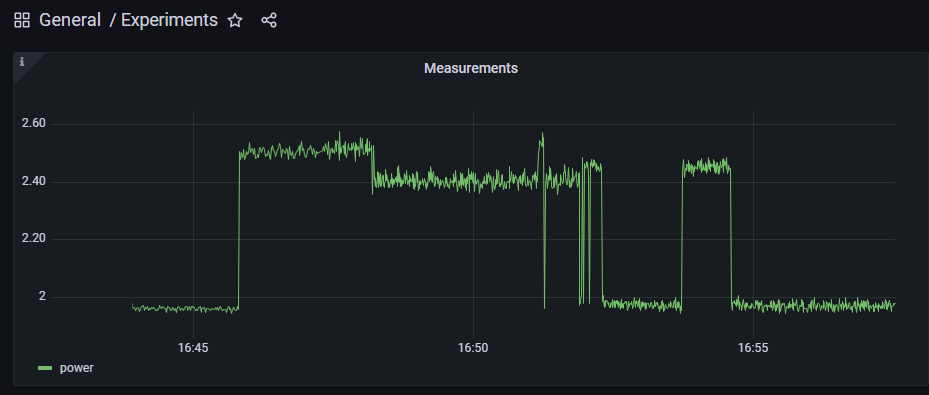
\includegraphics[width=\columnwidth]{Figures/rig/run1.png}
  \caption{Initial manual measurement run}
  \label{Run 1}
\end{figure}

\subsection{Application Comparisons}
\label{comparisons}

To demonstrate that the control and data collection aspects of the prototype apparatus were functioning correctly, a selection of common web server applications were compared. As of June 2023, the three most popular web servers were \emph{NginX}\footnote{\url{https://www.nginx.com/}}, \emph{Apache}\footnote{\url{https://httpd.apache.org/}}, and \emph{Cloudflare}\footnote{\url{https://www.cloudflare.com/}}, together serving over 50\% of the world's websites \citep{Netcraft2023}. \emph{NginX} and \emph{Apache} are open source software and were easily installed on the DUT. \emph{Cloudflare} is proprietary software, and was not available for download and installation, but it is apparently based on the \emph{NginX} codebase, so this was eliminated from the comparison.

Apache and NginX are general purpose web servers which can both serve pre-generated web pages from file and be configured to execute user code to respond to HTTP requests. Two other general purpose web servers were also evaluated: \emph{Lighttpd}\footnote{\url{https://www.lighttpd.net/}} and \emph{Caddy}\footnote{\url{https://caddyserver.com/}}. \emph{Lighttpd} is known for its speed \citep{Bogus2008}, but there was no information as to whether that would translate to lower energy usage. \emph{Caddy} is known for its extensibility, and has been used for a range of academic projects \citep{OCallaghan2017} \citep{Ardi2021}.

In some applications, a service requires dynamic generation of HTTP responses, for example a page containing information specific to the requesting user or providing an API which returns data calculated or retrieved from elsewhere. In such cases there are two broad approaches. One approach is to use a general purpose web server to handle the HTTP protocol and pass the request data on to the application code which acts as some form of `plugin' or `extension' to the web server. The other approach is to dispense with the general purpose web server and instead  for the application to handle the details of the HTTP protocol itself. To achieve this it is common to `embed' a specialist web server component or library into the application.

The energy usage of some well-known web server components was investigated, using each one to build a simple file-only server. Two programming languages were used which are popular for this kind of stand-alone web application development: \emph{Java}\footnote{\url{https://www.java.com/}} and \emph{Node.js}\footnote{\url{https://nodejs.org/en}}. With \emph{Java}, servers were built using both the web server code built in to the standard java libraries and a third-party web server component, \emph{Jetty}\footnote{\url{https://eclipse.dev/jetty/}}. For \emph{Node.js}, a server was built using the standard \emph{Express}\footnote{\url{https://expressjs.com/}} library. For the standard \emph{Java} and \emph{Express} applications, two versions were built, one which always serves the web content from files, and one which caches frequently requested data in memory. In \autoref{Server Energy}, the caching implementations are marked with \verb!(*)!

To compare the energy usage of the different web servers an example website was created with just one page. That page contains text and HTML markup as well as external images and CSS styling in a manner representative of a typical public `blog' page, so it requires multiple HTTP requests to fully render the resulting page. The \emph{Siege} load-generation software correctly recognises and fetches these external files to simulate a request from a real web browser. Before starting automated testing, each server was checked by requesting the example page using \emph{Chrome}\footnote{\url{https://www.google.com/intl/en_uk/chrome/}}, the web browser with the largest current market share \citep{StatistaBrowsers}. The resulting rendered page was observed to visually check that all page assets were correctly located and rendered. Where necessary, server configurations (in the case of the general purpose servers) and code (in the case of the server components) were adjusted until a successful page was achieved.

To determine the energy usage impact of an application running on a general-purpose web server, \emph{WordPress}\footnote{\url{https://wordpress.org/}} was installed into each of the general-purpose web servers. \emph{WordPress} is a `content management' application \citep{Patel2011a} estimated to run approximately 50\% of the world's websites \citep{W3Techs2022b}. The static files and the \emph{WordPress} application were configured to serve identical web pages. 

Once there was confidence that each web server was configured and working correctly, the automated energy usage measurements began. Each server was subjected to a load of 100 page requests while measuring the power used by the DUT. Each experiment was repeated several times to determine a range of energy usage and to reduce the impact of accidental or unrelated activity during measurement. For each experiment, the mean power usage in Watts was multiplied by the length of time it took for the application to handle the load in seconds to give a total energy usage in Joules. The results, showing ranges and mean values, are summarised in \autoref{Server Energy}.

\begin{figure}[htbp]
  \centering
  \includesvg[width=\columnwidth]{Figures/rig/energy.svg}
  \caption{Energy usage grouped by server}
  \label{Server Energy}
\end{figure}

In addition to measuring the energy usage during each experiment, the time it took for each of the servers to complete serving the requests from LOAD was also tracked. The results, laid out in the same framework as \autoref{Server Energy}, are shown in \autoref{Server Time}.

\begin{figure}[htbp]
  \centering
  \includesvg[width=\columnwidth]{Figures/rig/time.svg}
  \caption{Experiment duration grouped by server}
  \label{Server Time}
\end{figure}

\subsection{Analysis}

The most obvious observation from these results is that, in every case, WordPress consumes a lot more energy to serve the same website than any of the static servers. The median energy usage for all the WordPress experiments was 347J, while the median usage for the static servers was just 29J. That's roughly 12 times the energy to perform the same task. Comparing the median values does not tell the whole story, though. The purpose of this apparatus is to enable decisions to be made between alternate options with the aim of reducing overall energy usage. Comparing the `worst' approach in this group (\emph{WordPress} running on \emph{Caddy} with a mean energy usage of 413J) to the `best' (\emph{Lighttpd} serving static files with a mean energy usage of 12J) shows that \emph{WordPress} on \emph{Caddy} uses over 33 times more energy for this scenario.

The current hypothesis is that the extra energy used by the \emph{WordPress} servers is due to a combination of several factors. \emph{WordPress} is written in the \emph{PHP}\footnote{\url{https://www.php.net/}} programming language, known to consume more energy than the compiled languages typically used to write efficient servers \citep{Pereira2017} \citep{Pereira2021}, and which does not run natively in any of the servers investigated. Once an incoming HTTP request is received and decoded by the host server it must then be passed on, using one of a variety of methods, to a separate process responsible for running the \emph{PHP} code. When the \emph{PHP} code has completed processing the request, the response must be passed back to the host server and then returned to the client. All this communication takes resources. \emph{PHP} is a language which sits within HTML markup. To prepare a response, the \emph{PHP} processor must parse the combined file, execute any contained PHP code, which may in turn require the loading and execution of other \emph{PHP} files, and then combine the results and the original markup into a final web page. Depending on the configuration of the host server, this \emph{PHP} code may need to be fetched from files and re-parsed every time, or some or all of it may remain in memory. All this page loading and processing also consumes energy. In the particular case of \emph{WordPress}, much of the page content is stored in a database. To generate a response page requires not only all the processing described above, but also one or more requests to a database, all of which consumes yet more energy.

In contrast, the process for serving static websites is much simpler. A request is decoded and resolved to a filename. That file is then loaded, either from storage or from a memory cache, and returned as-is to the client. The experimental results show that this process clearly takes less energy than generating a \emph{WordPress} page on any server.

Although not explored in this research, technologies do exist to mitigate some of the issues of \emph{WordPress}. Typically these are positioned as ways to improve the response speed and throughput, but they are also likely to have an impact on energy usage. Plugins are available for WordPress which cache full or partial pages, eliminating the need for some of the database accesses and page construction \citep{BoldGrid2022}. However, such plugins are themselves written in \emph{PHP} so still suffer the issues of communication overhead and relatively slow, energy-intensive execution. Depending on the host server there may also be caching available at the request and response level, eliminating the need to invoke the \emph{PHP} code at all for some frequent requests. Caching is also possible in the network infrastructure between the client and the server \citep{Kusuma2017}. This is a common use-case for the \emph{Cloudflare} software mentioned in \autoref{comparisons} and contributes to its position in the server rankings. Finally, there are tools which can convert some kinds of \emph{WordPress} website to a static site. All of these techniques require some combination of extra configuration, installation of plugins \citep{Data2017}, and costs \citep{Strattic}, which limits their uptake. 

As mentioned in \autoref{comparisons}, \emph{Apache} and \emph{NginX} are currently the most used servers for general websites. Between these two the situation is more complex. When running \emph{WordPress}, the two are roughly similar. \emph{Apache} shows a lower mean energy usage, but a wider range. When serving static websites, \emph{NginX} is a clear winner with \emph{Apache} using roughly 2.7 times as much energy on average. Usage of \emph{NginX} is currently increasing, largely at the expense of Apache \citep{Netcraft2023}.

Of the four general-purpose web servers examined, the lowest energy usage in both static and \emph{WordPress} scenarios was \emph{Lighttpd}, averaging 286J for the \emph{WordPress} runs and 12J for the static website. This appears to validate the claim that \emph{Lighttpd} is faster, and also the assumption that this translates into using less energy to process the same load. Conversely, the worst server was \emph{Caddy}. Using roughly 6 times as much energy as \emph{Lighttpd} for the static scenarios and roughly 1.5 times as much for the \emph{WordPress} scenarios. \emph{Caddy} may be more extensible, but that comes at a cost.

The component-based servers all showed broadly similar energy consumption to NginX when used for static files. Not as good as \emph{Lighttpd}, which has obviously been highly tuned, but better than \emph{Apache} and \emph{Caddy}. There is a slight indication that caching frequently-used pages in memory improved the energy consumption of the \emph{Node.js} server, but had little effect for the \emph{Java} server. Further testing with a broader range of page requests would be needed to see if this holds for more realistic scenarios.

Of particular interest were the similarities and differences between the energy usage and speed of the different servers. Software performance, in the sense of speed to complete a task or throughput for non-completing services, is much more commonly measured than energy usage \citep{Freitas2014} \citep{Kuber2023}. In software the term \emph{efficiency} is almost universally considered in performance terms. Several researchers have attempted to determine a mathematical relationship between time performance and energy usage \citep{Kalaitzoglou2014a} \citep{Stoico2023}, in the hope of eliminating the need for costly energy measurement apparatus.

In both aspects the \emph{WordPress} servers were considerably worse than the static servers, with median duration of 412 and 213 seconds, respectively. The difference is not as great as the energy usage figures, however. The \emph{WordPress} servers show a similar pattern of better and worse. This might be taken to imply that experiment duration is a reasonable proxy for energy usage, at least for a simple `bigger or smaller' comparison. This relationship does not hold for the static servers, though. The component servers, which consumed roughly the same energy as \emph{NginX}, and less than \emph{Apache} and \emph{Caddy}, take over twice the time to service the same requests as \emph{NginX} and are considerably slower than both \emph{Apache} and \emph{Caddy}. Even within the general-purpose servers the relationship between performance and energy usage does not hold well. \emph{NginX} uses 3-4 times as much energy as \emph{Lighttpd} for roughly similar performance.

The apparent similarity between the performance of the component servers, despite being written in different programming languages and using a range of approaches, needs further research. There may be some underlying factor which is constraining their performance but does not apply to the general-purpose servers.

\section{Limitations and Drawbacks}
\label{limitations}

The apparatus and software described in this chapter have been developed as a prototype to investigate the feasibility of a low-cost way to include energy usage comparison in the normal process of software acquisition and development. However, this system differs in several key areas from the platforms in common use in commercial servers.

\subsection{Processor}

Raspberry Pi computers use 32 or 64-bit ARM \emph{Reduced Instruction Set Computer} (RISC) processors. While computers using such processors are becoming more popular in datacenters, they are still in a minority  \citep{Korolov2022}, with most servers using \emph{Complex Instruction Set Computer} (CISC) processors from Intel or AMD, even though switching to RISC processors could potentially provide equivalent performance at a reduced energy consumption \citep{Varghese2015}. The Raspberry Pi 4 used in this prototype has 4 CPU cores. This is the maximum for current Raspberry Pi devices, but Intel processors, for example, are available with tens \citep{Intel2022} or even hundreds \citep{Intel2023} of cores. Software which can make use of more CPU cores could exhibit a different energy usage profile when run on such processors \citep{Basmadjian2012}.

ARM processors are designed around a RISC model with relatively few processor instructions compared to equivalent designs from Intel and AMD. Specific implementations of the ARM processor core may have different amounts and speeds of local instruction and data cache and may include or omit features such as instruction look-ahead. These differences can affect both manual and automated code optimization strategies, and in turn may affect the performance of programming languages and applications \citep{Hartley2022}.

\subsection{Storage}

The initial choice of the Raspberry Pi Foundation to use SD cards as the sole form of persistent storage was unusual. With the exception of a few niche cases \citep{RaspberryHosting}, commercial servers use spinning hard drives or solid-state SSD or NVMe drives. SD cards are known for being slow in comparison with other forms of storage. Typical SD cards range from 5-15MB/s write speed compared to 160MB/s for a typical hard drive, 550MB/s for SSD, and 5000MB/s or more for NVMe \citep{Tekie.com}. Software which makes a lot of storage access may become \emph{IO bound} - unable to process data at full speed because it is waiting for the storage device - and therefore exhibit a different energy usage profile. SD cards are also known to be less reliable than the other forms, with some Raspberry Pi hosting companies allowing only network storage rather than support the risk of SD card failure \citep{MythicBeasts}

There are ways of connecting other forms of storage to the Raspberry Pi. Every Raspberry Pi has USB ports, and on the Raspberry Pi 4 two of those are USB3 and therefore theoretically capable of up to 5GB/s. In practice the available speed will depend on both the type of drive and the protocols supported by the USB drive controller, as well as the internal architecture of the Raspberry Pi 4 which shares a single 4GB/s PCIe lane between all the USB ports. Network storage is also a possibility. Modern Raspberry Pi devices can be configured to boot and operate entirely from network storage \citep{RaspberryPiFoundation2023}. As this apparatus is intended for network-driven stress testing, It was considered that the extra network traffic associated with storage access might affect the performance and thus the power usage readings. Both USB storage and network storage have a bigger problem for this application, though. Many USB hard drives and network storage devices require more power than the Raspberry Pi is able to provide, which means that they would need an external power source. This would exclude any power usage associated with storage from the results and act against the intention to perform a holistic measurement.

Possible ways around this limitation are discussed in \autoref{Improvements}.

\subsection{Memory}

The Raspberry Pi is an all-in-one single-board computer. The amount of memory is fixed at time of manufacture and the current maximum is 8GB. While this is enough for simple or undemanding applications it is not representative of many real systems. Commercial servers are commonly available with as much as 256GB of memory \citep{FastHosts2023}. Any software which requires more than the available memory on the Raspberry Pi board will either fail to operate or suffer changes to its performance and energy usage.

\subsection{Apparatus software}

The software used both for running the application being tested and for providing representative usage are unlikely to be identical to those found `in the wild'. The current approach to simulating usage is simplistic and repetitive and therefore does not execute a wide variety of code and data in the application being measured. This has the specific side effect that applications which cache frequently requested data can quickly `warm up' and may exhibit different performance and power usage than if they were receiving a broader and less predictable range of requests. Note however, that the LOAD software makes use \emph{Siege}\footnote{\url{https://github.com/JoeDog/siege}}, an open source load tool of the type commonly used for performance and functionality testing during development, so this problem is not unique to this apparatus.

The software for starting. stopping, and measuring idle power consumption of applications is also relatively simplistic. Applications to be tested are started by shell scripts which may not accurately match the real-world installation and start-up process. Applications are left running only for the duration of their measurement cycle which may mask longer-term caching, secondary compilation, and other performance strategies. Supporting services such as databases may or may not continue running after a measurement run is complete, depending on how they have been installed, and this may affect the measurement of idle power consumption and even possibly the active power consumption of later applications.

\subsection{Reflections}

It is clear, for all the reasons mentioned above, that the prototype apparatus is far from identical to real software deployments. Whether it is representative enough to be useful is a different question. The aim of the apparatus is not to provide an accurate \emph{absolute} measurement of the energy used by a particular installation of software. Instead, the aim is to enable \emph{comparisons} between different pieces of software. Such comparisons are useful both when choosing between candidate software components or applications, and when comparing different versions of the same software as part of development. In either case, the apparatus provides a relatively consistent environment for such comparison. A similar approach is commonly used when testing software functionality and performance during development \citep{Collins2012}. Such tests are performed in a `test environment' or `development environment' which may be smaller or otherwise different from the live deployment.

It is suggested that if software \emph{A} runs correctly and uses less energy than software \emph{B} for a similar task when measured on this apparatus, it can be taken as an indication that it is likely to use less energy when deployed live. Such information is potentially very useful and otherwise hard to obtain.

\section{Improvements and Future Possibilities}
\label{Improvements}

\subsection{Addressing Limitations}

A prototype is not a finished product, and exists as much to discover limitations and provoke suggestions for improvements as it does to validate an idea. As can be seen from \autoref{limitations}, this prototype apparatus has several aspects in which it may not be fully representative of a real deployment environment.

Some limitations of the prototype could be partially mitigated without major changes. For example, the speed and reliability issues associated with SD cards could be improved by sourcing high-speed USB storage with low enough power requirements that it can operate as the primary storage for the DUT and LOAD devices. Likewise, the issue of a simplistic and potentially unrepresentative pattern of requests from LOAD to DUT could be addressed by finding or creating a more sophisticated load service.

Other limitations would require larger changes to the hardware of the apparatus. The largest change would be to replace the Raspberry Pi with an alternate platform which addresses some or all of the limitations of that device. Several manufacturers now produce equivalent single-board computers with a range of memory and storage options. Most also use ARM processors, but some are available with Intel, AMD, or Risc-V processors instead. In most cases, features such as larger memory, more CPU cores, or on-board SSD or NVMe storage also increase the power consumption and price of these devices. After this research took place, a fifth iteration of the Raspberry Pi was released which includes a relatively high-speed PCI interface. Several after-market adapter boards are now available which allow the connection of NVMe storage which is more representative of common server deployments.

The popularity of USB Power Delivery (PD) for charging mobile devices has also led to an uptake in the use of USB PD for general computer use. An increasing number of laptop and `mini PC' devices now use this standard for operational and battery charging power. Replacing the DUT with such a device might be physically cumbersome, but should pose no major software or operational issues. The prototype apparatus is capable of measuring power usage of any device using USB PD up to version 3.0. However, version 3.1, introduced in 2021, allows voltages up to 48V which are beyond the range of the INA260 power measurement chip.

Any changes to the power supply to the DUT device would probably also require the separation of power supplies. In this prototype, DUT, LOAD, and CTRL are all powered by a single stable 5V supply. USB PD includes a negotiation process and is therefore only suitable for a single device at a time. If just the DUT device requires USB PD, then potentially LOAD and CTRL could still share a 5V supply.

The current prototype does not use all the features of the INA260 measurement chip. It is possible that the accuracy of the readings could be improved by, for example, using the power usage calculated by the INA260 directly rather than the existing approach of measuring voltage and current and combining them to derive the power.

To support DUT devices requiring higher DC voltage and current, or even an AC supply, would require a different power measurement technology. Integrated circuits, boards, and full devices are assailable from a variety of manufacturers, but these would represent a major change to the prototype apparatus and would also potentially increase its cost.

\subsection{Software Improvements}

As well as addressing the differences between environments, there are other potential software changes which could improve the usability and effectiveness of the prototype. For example, the need to manually adjust the SD card `disc' image for each of the Raspberry Pi devices is intrusive and error-prone. There are several potential ways to address this including: storing some form of role ID in the Raspberry Pi EEPROM so it persists between SD card changes; placing `jumpers' or other connectors on the Raspberry Pi GPIO pins which can be read on start-up; requiring a USB `key' to identify the device role; and so on. While such changes would be an improvement, they are dependent on the hardware of the raspberry Pi, and would be unlikely to work if a different device were to be used instead.

The current prototype software makes the assumption that an application running on the DUT, but receiving no requests from LOAD, uses negligible energy. This has been observed to be the case for the small number of applications investigated so far, but arguably may not be the case for all applications. To address this oversight, there should be the option to measure the baseline energy usage before instructing the DUT to \emph{Warmup}.

This prototype has so far only been used with a small range of applications which were manually installed prior to measurement. \emph{Warmup} and \emph{Cooldown} scripts were also created by hand. This approach is not suitable for an environment requiring more frequent or varied, automated, measurements. The addition of an \emph{install} and \emph{uninstall} steps to the measurement process would allow, for example, a call to an external API or webhook which would then manage the installation without the measurement software needing to know the details. When the installation step is complete, the system can proceed with the rest of the measurement cycle, then notify the external system to undo the installation in the same way.

\subsection{Future Possibilities}

The current prototype embodies a relatively simple model of a single apparatus testing the overall energy usage of a single application at a time. While this functions as a proof of concept, there are ways in which this model could be enhanced to be easier to use, provide more precise information, and scale more effectively to larger and more complex systems.

A relatively simple enhancement would be to support multiple installations of the measurement apparatus communicating with a shared LOG service and database. This would require the provision of a unique identifier to each apparatus, and that id to be included in all messages to the database. The apparatus id would then be stored with the status updates and readings in the database, enabling analysis to be performed either on the results of a specific apparatus or aggregated across all installations. A system such as this would allow either parallel evaluation of the same measurements on multiple candidate applications or simultaneous evaluation of multiple different load patterns on a single application.

At the moment the prototype software treats all power measurements during a run as relating to a single session. The assumption is that the load client generates `realistic' load which can be used to measure the power consumption of the application under representative usage. The collected results can then be used to statistically determine values such as the the total, average, and peak energy usage for the scenario. While this is arguably useful, it is not particularly fine-grained. To measure any different scenario requires a complete test run including \emph{warmup}, \emph{cooldown}, baseline measurements, and potentially also installation and removal of the software being tested. An alternative approach would be to split the main phase of the measurement, once the baseline measurement has completed, into distinct sections representing different volumes or patterns of load. This could potentially speed up the process and allow a greater variety of measurements in a given time.

In agile software development, software is typically tested many times and at many levels during development, not just when an application is complete \citep{Fowler2012}. When evaluating potential third-party code, components, or libraries to include in an application, it would be useful to be able to evaluate the relative energy consumption of the alternatives. In both these cases, the code to be evaluated is not in the form of a whole application service which exposes an API for a load client to exercise. Instead, the system needs to evaluate fragments of software. This is a more complex challenge. One approach is to build a `wrapper' application to contain the software fragments and translate client API requests into internal software calls. This has the advantage of fitting well with the existing architecture, but for some components the overhead of the containing application could outweigh the energy usage of the components. An alternative approach is to exercise the software from within the DUT device without the overhead of processing network requests. While this could be more effective, it would require changes to the architecture to ensure that measurement readings and status notifications to the LOG database are correctly synchronised.

The current prototype apparatus was designed for low cost and ease of construction and testing. More work would be needed to produce a version which would be suitable for inclusion in commercial build processes. The hardware would need to be self-contained, robust, maintainable, and protected from accidental damage. The software would need to be flexible to support unknown future applications and usable without the need to make internal changes. The improved hardware would require sourcing of components and a casing as well as physical and electrical testing. The software changes would require improving the architecture to support configurations, plugins, or `hooks' to integrate with existing test and application infrastructure.

\subsection{Further Research}

The development of this prototype is continuing. Research plans include: evaluating alternative platforms to the Raspberry Pi; evolving the hardware and software into a self-contained software energy measurement appliance; and running trials of the apparatus with existing software build and test processes.

Further research is also needed in the broader field of software energy usage measurement and communication. The results of energy usage of different software applications and components need to be disseminated so that potential users can make an informed choice. This would need standards and repeatable methodologies as well as devices such as this prototype apparatus.

\section{Conclusions}
\label{Conclusions}

The primary purpose of this research was to determine if the energy usage of software applications and components varies, and therefore whether selecting a more energy-efficient combination of components would show an overall reduced energy use compared with an application constructed using less energy-efficient components. Arguably this has been shown to be the case, and the results illustrate measurable variation in the energy usage of different software applications which perform similar functions.

The energy usage results from the web server comparisons showed considerable differences in energy usage and performance between candidates. The energy usage results from experiments using \emph{WordPress} software are considerably higher than those from a static website with a similar appearance and functionality. Further research is needed to validate these results in real deployments, but initial indications are that application energy consumption can be reduced by switching to a more energy-efficient web server application and that a large amount of energy, with its associated greenhouse gas emissions, could be saved by switching to static websites wherever possible.

The secondary purpose of this research was to determine whether a low-cost apparatus could be constructed and used to compare the relative energy usage of different software. An apparatus was successfully constructed and used to compare a variety of software applications. A low-cost apparatus of this nature could therefore be useful both for selecting between functionally equivalent software applications, and for tracking and addressing changes in energy usage between releases of software during development.

This research also highlights the variable relationship between performance and energy usage. Although the same word `efficiency' is used in both cases, the meaning and the measurements can be very different. The amount of energy used by an application to perform a particular task depends on many factors including programming language, application architecture, and the use of libraries and components. Performance measurement, along with other estimation techniques such as static analysis, is not a reliable method of determining energy usage.

This prototype apparatus demonstrates that the concept of low-cost automated energy usage comparison is valid, but there are also ample opportunities for improvement and further research. It is hoped that energy usage comparison will soon become a common part of both the software acquisition and software development processes.
